% !TEX root = ../../I4PRJ, Grp3 - Rapport.tex
\subsubsection{Implementering}
Den visuelle Implementering af websitet med ASP.NET MVC, den visuelle implementering er skrevet i HTML og CSS. Clientside funktionaliteten er skrevet i JavaScript slutteligt er der brugt razor, som er et server-side markup sprog.

\begin{figure}
	\centering
	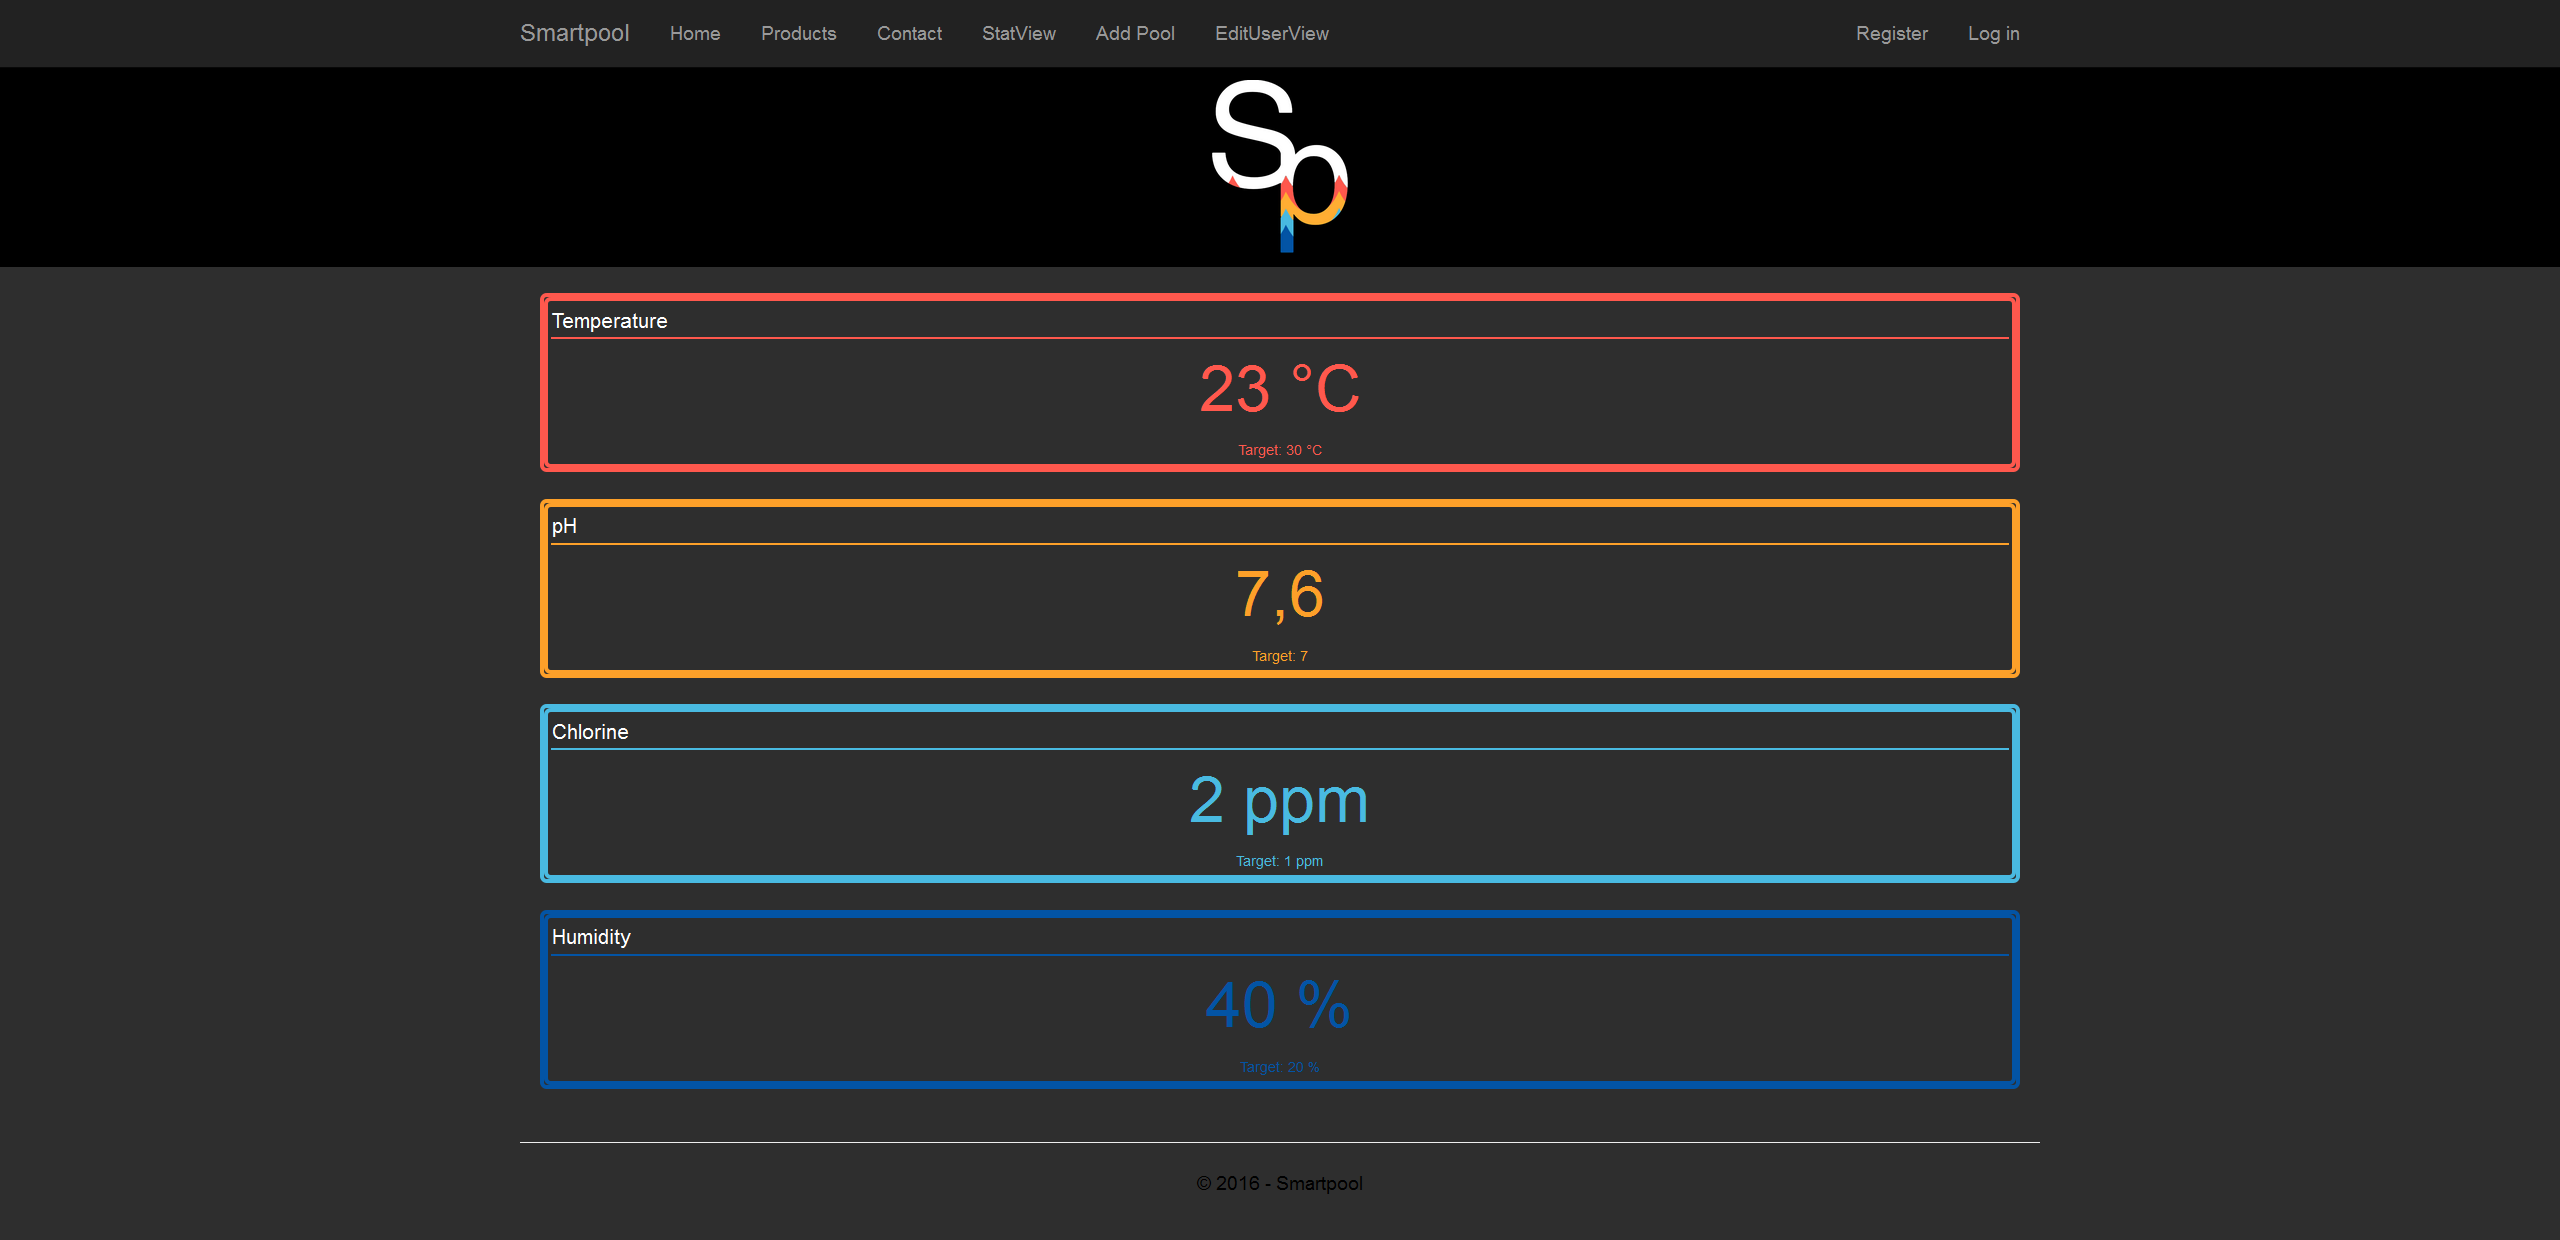
\includegraphics[width=1.0\linewidth]{figs/implementering/web_statview}
	\caption{Web StatView}
	\label{fig:webstatview}
\end{figure}

\paragraph{LoginView}
LoginView ses på figuren nedenfor:

\begin{figure}
	\centering
	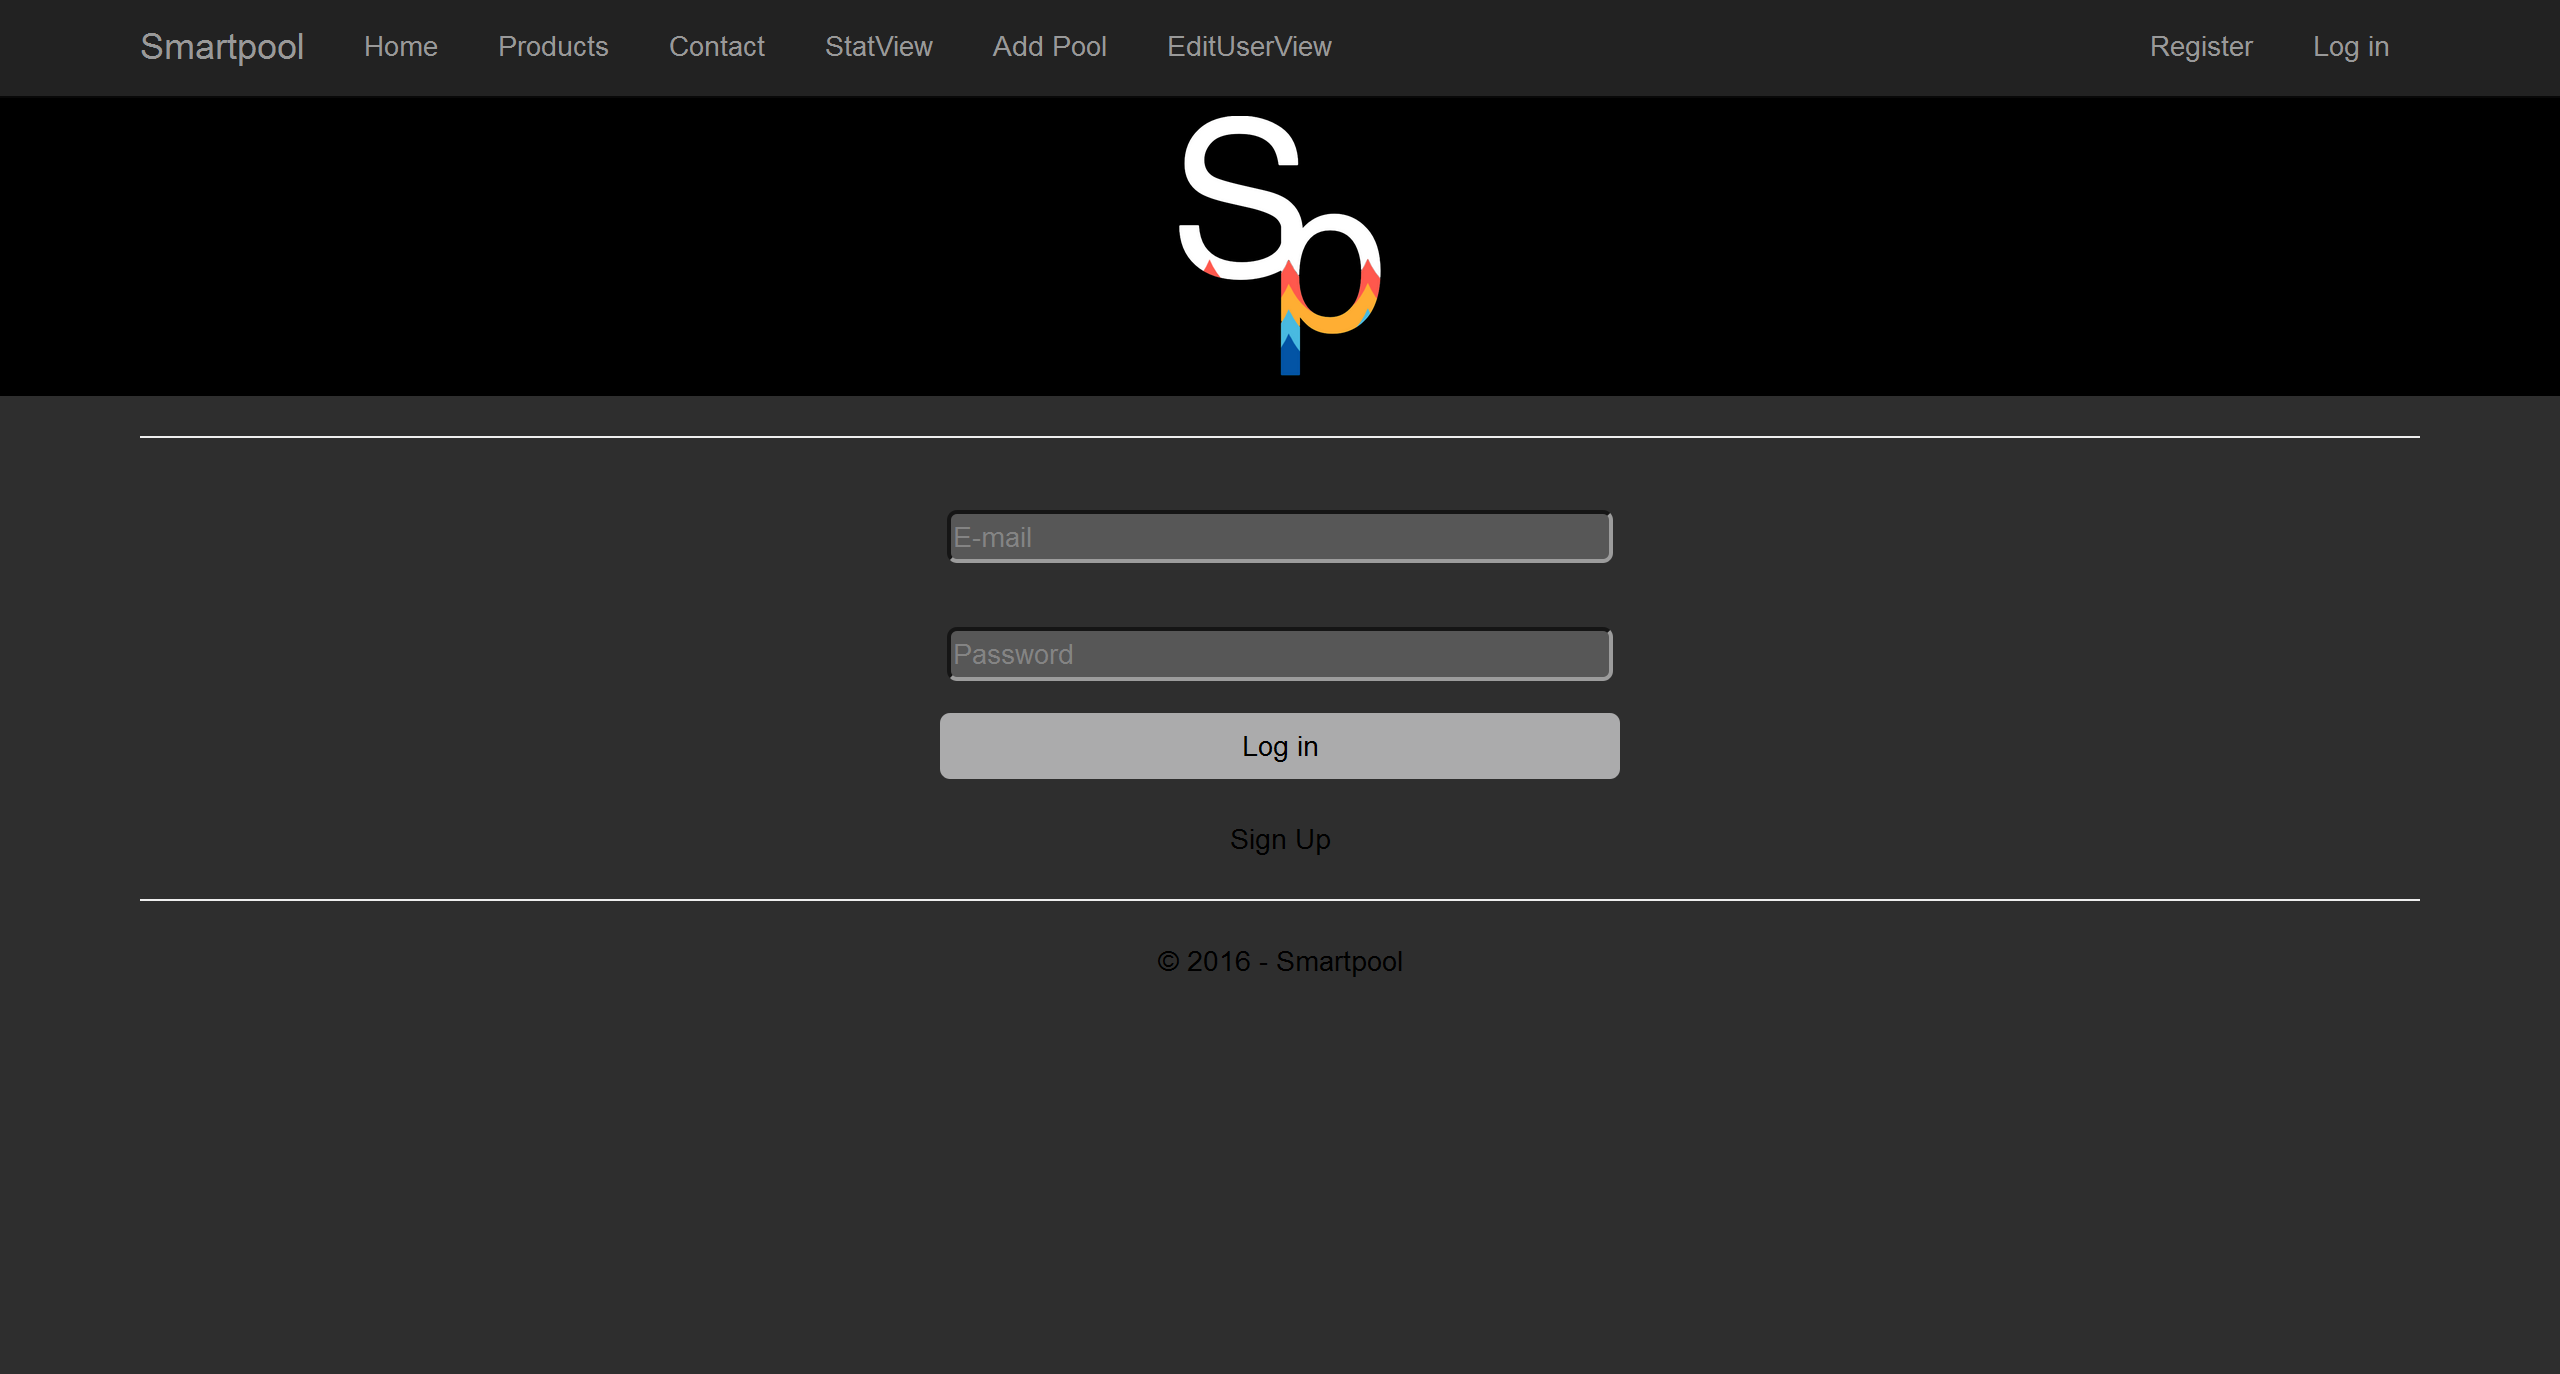
\includegraphics[width=1.0\linewidth]{figs/implementering/web_login}
	\caption{Web LoginView}
	\label{fig:webloginview}
\end{figure}

For at logge ind på serveren laves en 'Task' login.

\begin{lstlisting}[caption=Login, label=code:Login]
 // POST: /Account/Login
        [HttpPost]
        [AllowAnonymous]
        [ValidateAntiForgeryToken]
        public async Task<ActionResult> Login(LoginViewModel model, string returnUrl)
        {
            var loginController = Controller as ILoginViewController;
            loginController.DidChangeEmailText(model.Email);
            loginController.DidChangePasswordText(model.Password);
            loginController.ButtonPressed(LoginViewButton.LoginButton);

            _returnUrl = returnUrl;

            return View(model);
        }
\end{lstlisting} 

Funktionen sender request til server ved Button.Pressed. Funktionen LoginAccepted kaldes når serveren svarer tilbage.

\begin{lstlisting}[caption=LoginAccepted, label=code:LoginAccepted]
public void LoginAccepted()
        {
            ActionInvoker.InvokeAction(ControllerContext, "RedirectLogin");
        }
\end{lstlisting}

LoginAccepted 'Invoker' et ActionResult RedirectLogin.
 
 \begin{lstlisting}[caption=Redirect Login, label=code:redirectlogin]

        [AllowAnonymous]
        public ActionResult RedirectLogin()
        {
            return RedirectToLocal(_returnUrl);
        }
        }
\end{lstlisting}

RedirectLogin redirects til en anden side på serveren når login accepteres.

\paragraph{AddPoolView}
AddPoolView ses på figuren nedenfor:

\begin{figure}
	\centering
	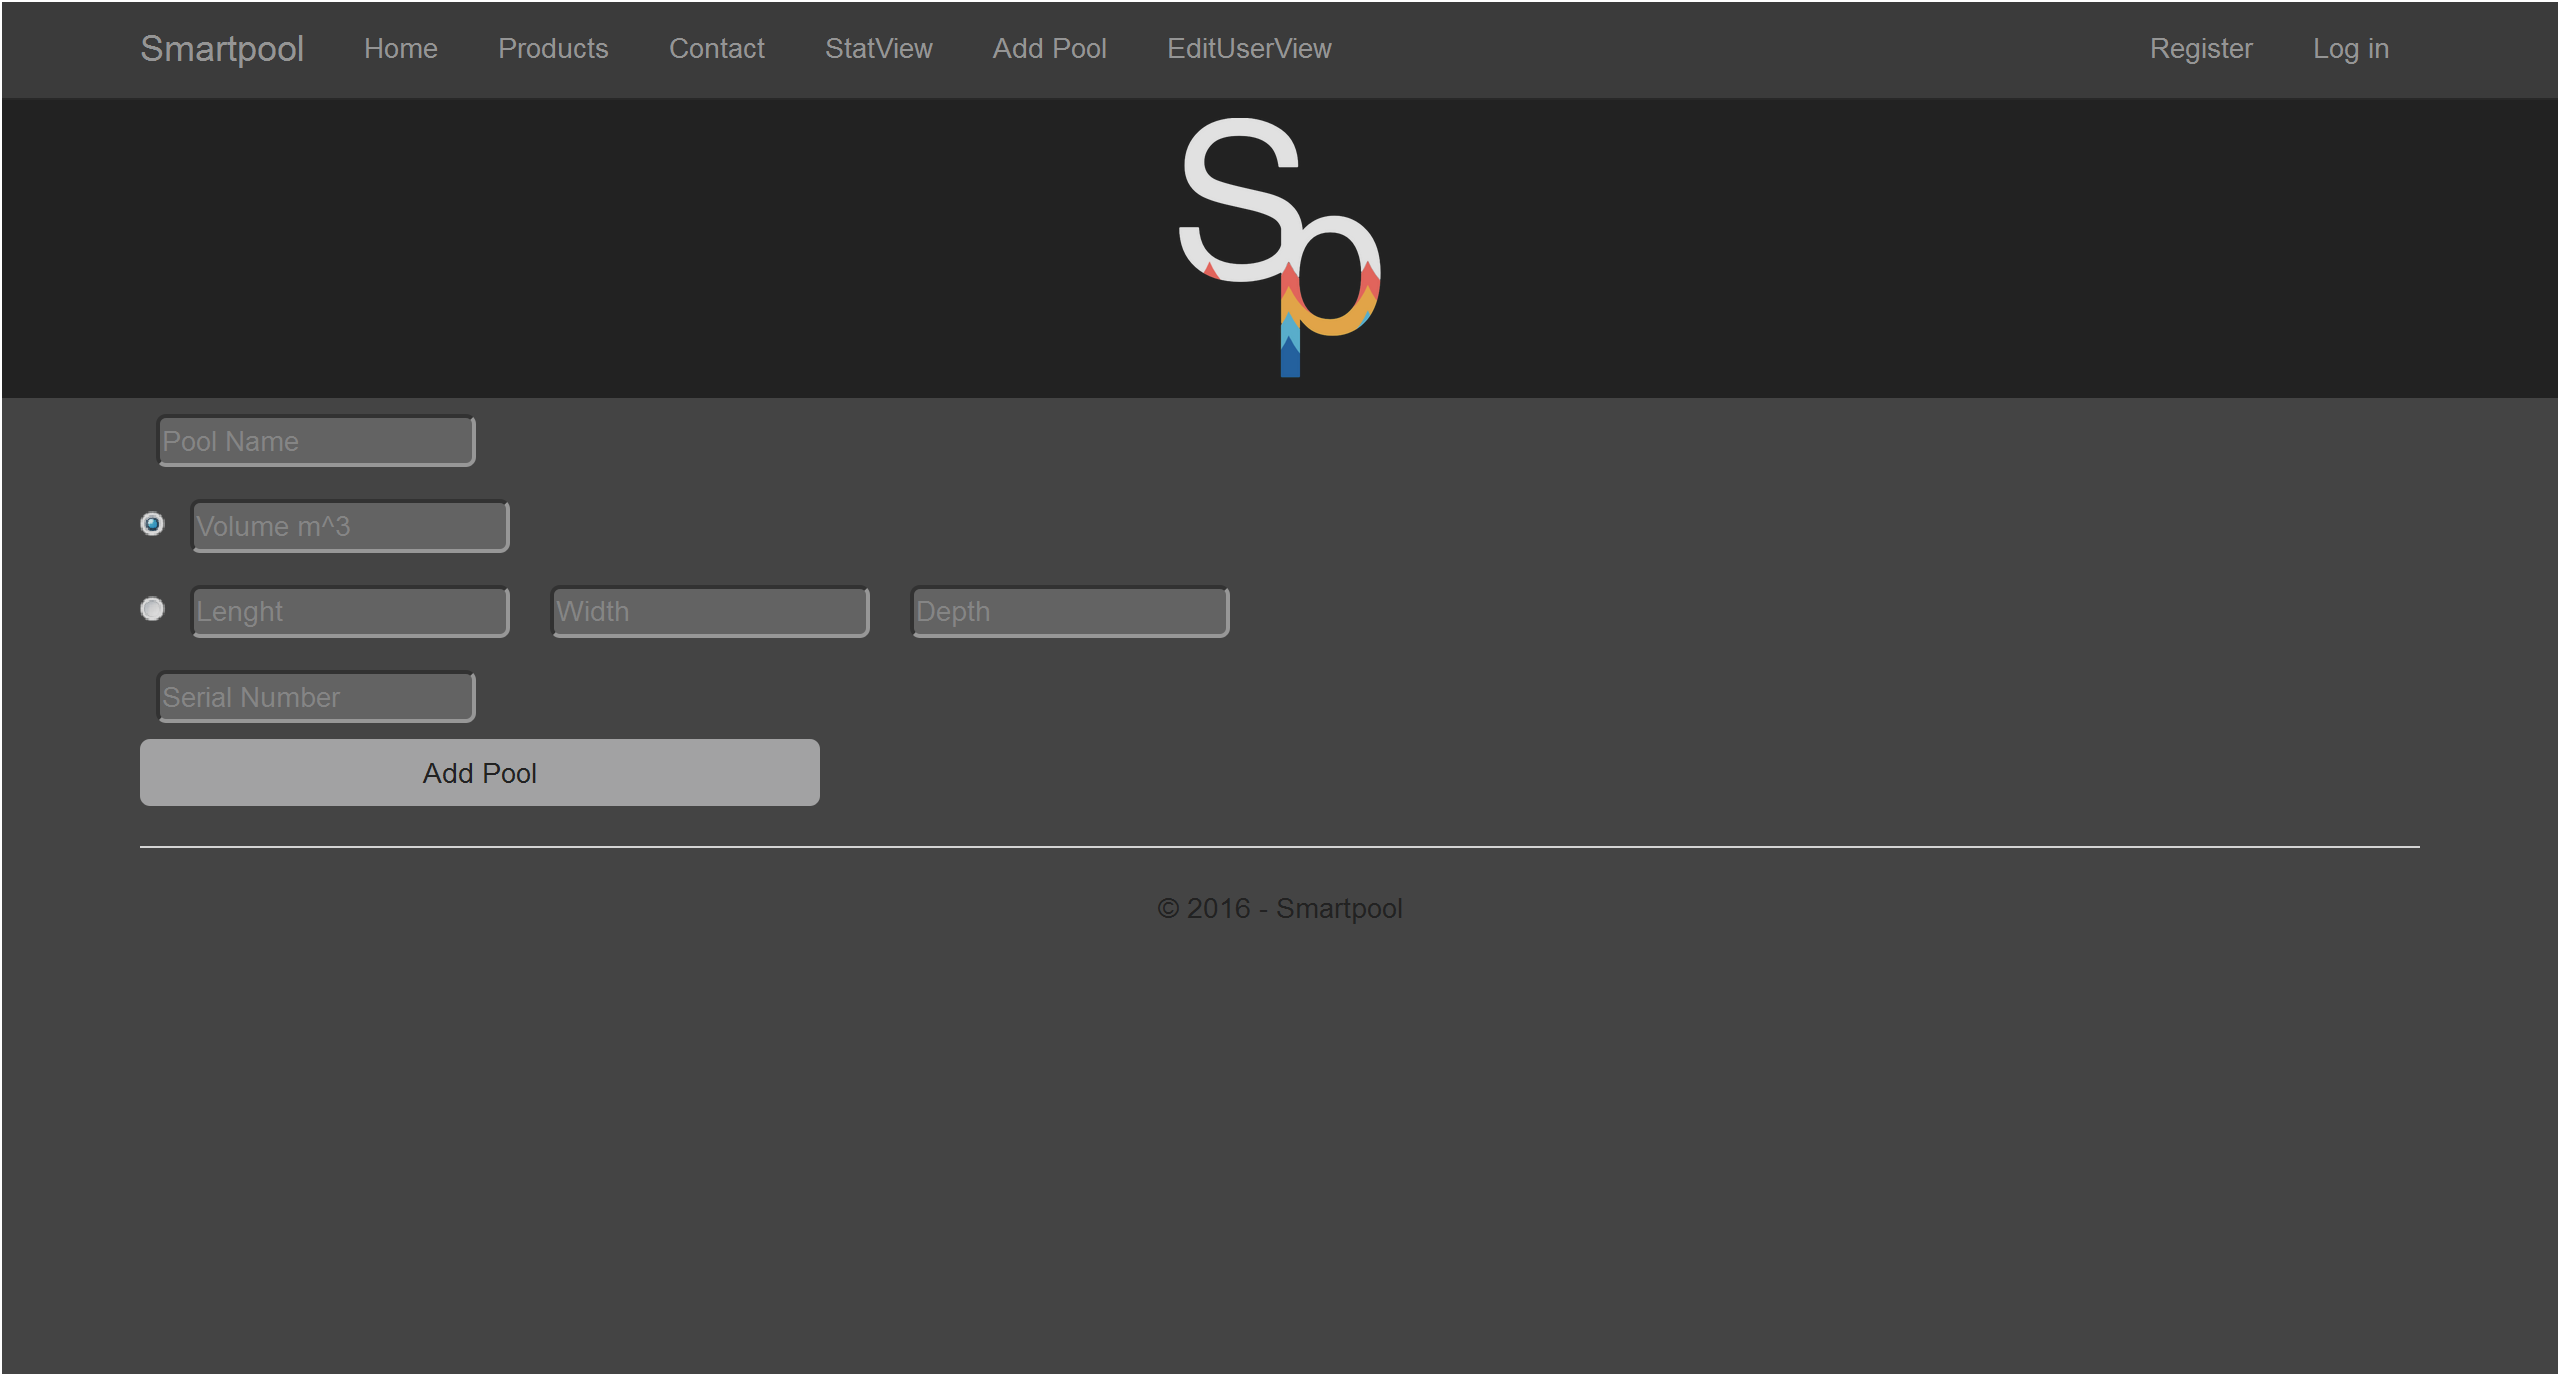
\includegraphics[width=1.0\linewidth]{figs/implementering/web_addpoolview}
	\caption{Web AddPoolView}
	\label{fig:webaddpoolview}
\end{figure}

Brugeren kan vælge enten at indtaste volumen eller dimensioner, ved at vælge på radioknapperne. Når den ene er valgt skal den anden mulighed ikke være tilgængeligt. Der håndterer scriptet enableTxtBox. Er brugeren begyndt at indtaste volumen, men ombestemmer sig, så skal tekstfeltet tømmes, det håndteres af scriptet clearText. Der er ikke muligt for brugeren at indtaste andet end tal, det håndterer scriptet isNumber. Alle scripts set i kodeudsnittet nedenfor.

\begin{lstlisting}[caption=AddPoolScripts, label=code:scripts]
 <script>
	function enableTxtBox1()
	{
         	document.getElementById("text1").disabled = !document.getElementById("radio1").checked;
         	document.getElementById("text2").disabled = document.getElementById("radio1").checked;
         	document.getElementById("text3").disabled = document.getElementById("radio1").checked;
         	document.getElementById("text4").disabled = document.getElementById("radio1").checked;
    }
</script>

<script>
	function clearText()
	{
		if(!document.getElementById("radio1").checked) text1.value="";
		if(document.getElementById("radio1").checked) {
         	text2.value="";
         	text3.value="";
         	text4.value="";
         }
    }
</script>

<script>
function isNumber(evt) {
    evt = (evt) ? evt : window.event;
    var charCode = (evt.which) ? evt.which : evt.keyCode;
    if (charCode > 31 && (charCode < 48 || charCode > 57)) {
        return false;
    }
    return true;
}
</script>
\end{lstlisting} 

For implementering af andre views henvises til projektdokumentationen. 


